% 行列投影迭代法：Kaczmarz与扩展Kaczmarz
\chapter{行列投影迭代法}
\label{sec:ls-row-projection}
\label{chap:row-projection-methods}

第~\ref{chap:stationary-iterations}章的定常迭代和第~\ref{chap:krylov-methods}章的Krylov方法，每轮都要用到整个矩阵，至少作一次矩阵乘向量。有些问题的数据却只方便逐行读取：观测按行陆续到达，或者矩阵太大，只能每次取出其中一行。这时自然的想法是每次只让一个方程成立，用一系列局部修正逐步逼近解。本章研究这种做法能求出什么解、何时收敛，以及方程不相容时应当怎样修改。

第~\ref{sec:ls-kaczmarz}节的Kaczmarz算法把当前解投影到所选方程的解超平面上，适用于相容方程；零初值时，它收敛到第~\ref{chap:linear-solution-selection}章的最小范数解。方程不相容时，各行没有公共解，单纯的行投影不会停在最小二乘解上。第~\ref{sec:ls-extended-kaczmarz}节的扩展Kaczmarz算法再用列投影估计右端中无法拟合的部分，把问题改写成相容方程后继续作行投影。

两种算法的推导都只用到超平面上的最短修正，即第~\ref{sec:ls-orthogonal-projection}节的正交投影；收敛分析用到伪逆、行空间与零空间的正交分解，以及第~\ref{chap:singular-value-decomposition}章中谱范数与最小正奇异值的刻画。本章$\bm A\in\mathbb R^{m\times d}$不必是方阵，两种算法都以$\bm A,\bm b$为输入、以$\bm x$为输出，投影中的残差和辅助向量只是内部状态。

\section{Kaczmarz算法}
\label{sec:ls-kaczmarz}

\term{Kaczmarz算法}（Kaczmarz method）每次只读取一行，把当前解修正到满足这一行的最近点。本节先由最短修正推导一次行投影，再说明怎样依次处理各行；算法实现在贯穿例上逐步执行循环版本；算法分析证明它在相容方程上的收敛，讨论随机选行，并说明它为什么不能直接处理不相容方程。

\subsection{主要思想}

要解的是方程组$\bm A\bm x=\bm b$，其中$\bm A\in\mathbb R^{m\times d}$，本节先设方程相容。记第$i$行为$\bm a_i^\top$，其中$\bm a_i\in\mathbb R^d$是列向量，方程组就是$m$个标量方程
\[
 \bm a_i^\top\bm x=b_i\qquad(i=1,\ldots,m).
\]
非零行的方程的解集是以$\bm a_i$为法向量的超平面，原方程的解就是这些超平面的公共点。每次只能读取一行时，一步能利用的只有一个方程，所以先回答：怎样修正当前点，才能使所选的这个方程成立。

\paragraph{满足一行的最短修正}
给定当前点$\bm x_k$与所选的行$i$，要找修正$\bm\delta$，使新点$\bm x_k+\bm\delta$满足第$i$个方程。把$\bm a_i^\top(\bm x_k+\bm\delta)=b_i$移项，得
\[
 \bm a_i^\top\bm\delta=s,\qquad s=b_i-\bm a_i^\top\bm x_k .
\]
$s$是第$i$个方程在当前点的残差，称为\emph{行残差}。$d\geq2$时，满足这个条件的修正有无穷多个。其余的行暂不考虑，取其中欧氏范数最小的一个，使新点尽量少偏离当前点。

先在例~\ref{ex:ls-stationary-running-example}的第一行上看这个最小化怎样求解。这一行为$\bm a_1=(4,1)^\top$，$b_1=1$，条件是$4\delta_1+\delta_2=s$。平面上与$(4,1)^\top$正交的方向是$(-1,4)^\top$，任何修正都可以唯一地写成
\[
 \begin{bmatrix}\delta_1\\\delta_2\end{bmatrix}
 =\gamma\begin{bmatrix}4\\1\end{bmatrix}+t\begin{bmatrix}-1\\4\end{bmatrix}.
\]
代入条件，正交方向的贡献$-4t+4t$相消，只剩
\[
 4\delta_1+\delta_2=17\gamma=s ,
\]
所以$\gamma=s/17$由条件确定，而$t$可以任取。修正的长度平方为
\[
 \delta_1^2+\delta_2^2=(4\gamma-t)^2+(\gamma+4t)^2=17\gamma^2+17t^2 ,
\]
交叉项$-8\gamma t+8\gamma t$同样相消。$\gamma$已经确定，长度在$t=0$时最小，最短修正是
\[
 \bm\delta=\frac{s}{17}\begin{bmatrix}4\\1\end{bmatrix}.
\]
它沿第一行的法向，系数等于行残差除以$\lVert\bm a_1\rVert_2^2=17$。

一般情形的推导相同。把任意修正分为沿$\bm a_i$的分量和与$\bm a_i$正交的分量：
\[
 \bm\delta=\gamma\bm a_i+\bm w,\qquad \bm a_i^\top\bm w=0 .
\]
行约束只涉及第一部分，给出$\gamma\lVert\bm a_i\rVert_2^2=s$。由勾股关系，
\[
 \lVert\bm\delta\rVert_2^2=\gamma^2\lVert\bm a_i\rVert_2^2+\lVert\bm w\rVert_2^2 ,
\]
它在$\bm w=\bm0$时最小。于是得到Kaczmarz更新
\begin{equation}
 \bm x_{k+1}=\bm x_k+\frac{b_i-\bm a_i^\top\bm x_k}{\lVert\bm a_i\rVert_2^2}\,\bm a_i .
 \label{eq:ls-kaczmarz-update}
\end{equation}
式中分子是行残差$s$，衡量当前点离满足第$i$个方程还差多少；除以$\lVert\bm a_i\rVert_2^2$，把这个差换算成沿$\bm a_i$的系数$\gamma$，它由法向量的长度决定，不是另外选取的步长；修正方向$\bm a_i$是超平面的法向。代回所选的行，
\[
 \bm a_i^\top\bm x_{k+1}=\bm a_i^\top\bm x_k+(b_i-\bm a_i^\top\bm x_k)=b_i ,
\]
这一行精确成立。新点是超平面上离$\bm x_k$最近的点，即$\bm x_k$到该超平面的正交投影（第~\ref{sec:ls-orthogonal-projection}节），所以这一步称为\emph{行投影}。

例中从$\bm x_0=\bm0$出发，第一行的行残差为$s=1-0=1$，投影后得
\[
 \bm x_1=\frac1{17}\begin{bmatrix}4\\1\end{bmatrix},
\]
可以核对$4\cdot\tfrac4{17}+\tfrac1{17}=1$。

\paragraph{依次处理各行}
一次行投影只照顾所选的一行，其他行可能因此失配。例中接着对第二行$\bm a_2=(1,3)^\top$、$b_2=2$作行投影：行残差为$2-(4/17+3/17)=27/17$，$\lVert\bm a_2\rVert_2^2=10$，得
\[
 \bm x_2=\frac1{17}\begin{bmatrix}4\\1\end{bmatrix}+\frac{27}{170}\begin{bmatrix}1\\3\end{bmatrix}=\frac1{170}\begin{bmatrix}67\\91\end{bmatrix}.
\]
这时第二个方程成立，第一个方程的左端却变成
\[
 4\cdot\frac{67}{170}+\frac{91}{170}=\frac{359}{170}\neq1 .
\]
所以只把每行投影一次是不够的，要反复访问各行。

访问的顺序有两种常用规则。\emph{循环版本}按$1,\ldots,m$的固定顺序重复遍历非零行，遍历一次称为一轮\emph{扫掠}。\emph{随机版本}每次按概率
\begin{equation}
 p_i=\frac{\lVert\bm a_i\rVert_2^2}{\lVert\bm A\rVert_F^2}
 \label{eq:ls-kaczmarz-row-probability}
\end{equation}
独立选取一行，较长的行被选中的机会较大；本节算法分析中的“随机选行”一段说明为什么这样取概率。两种规则的投影公式相同，都是式~\eqref{eq:ls-kaczmarz-update}。

\paragraph{到精确解的距离}
上例中第一个方程虽然重新失配，近似解却离精确解更近了。这一点对一般的相容方程都成立。任取一个精确解$\bm y$，由$\bm a_i^\top\bm y=b_i$，行残差可以写成$s=\bm a_i^\top(\bm y-\bm x_k)$，更新便成为
\begin{equation}
 \bm x_{k+1}-\bm y=\bm P_i(\bm x_k-\bm y),\qquad \bm P_i=\bm I-\frac{\bm a_i\bm a_i^\top}{\lVert\bm a_i\rVert_2^2},
 \label{eq:ls-kaczmarz-error-map}
\end{equation}
其中$\bm P_i$是到$\bm a_i^\perp$的正交投影。行投影去掉了$\bm x_k-\bm y$沿$\bm a_i$的分量，这个分量的长度为$|s|/\lVert\bm a_i\rVert_2$。由勾股关系，
\begin{equation}
 \lVert\bm x_{k+1}-\bm y\rVert_2^2=\lVert\bm x_k-\bm y\rVert_2^2-\frac{(b_i-\bm a_i^\top\bm x_k)^2}{\lVert\bm a_i\rVert_2^2}.
 \label{eq:ls-kaczmarz-distance}
\end{equation}
所以每一步到每个精确解的距离都不增，所选行的残差越大，距离减少得越多。距离减少并不意味着其他各行的残差都减少：投影只照顾所选的一行，已经满足的行可能重新失配，上例的第一个方程就是这样。

例中的精确解为$\bm x_\star=(1/11,7/11)^\top$，初始距离平方为
\[
 \lVert\bm x_0-\bm x_\star\rVert_2^2=\frac{50}{121}.
\]
由式~\eqref{eq:ls-kaczmarz-distance}，两步的减少量分别为
\[
 \frac{1^2}{17}=\frac1{17},\qquad \frac{(27/17)^2}{10}=\frac{729}{2890},
\]
于是
\[
 \begin{aligned}
 \lVert\bm x_1-\bm x_\star\rVert_2^2&=\frac{50}{121}-\frac1{17}=\frac{729}{2057},\\
 \lVert\bm x_2-\bm x_\star\rVert_2^2&=\frac{729}{2057}-\frac{729}{2890}=\frac{35721}{349690}.
 \end{aligned}
\]
三个点到$\bm x_\star$的距离依次约为$0.643$、$0.595$、$0.320$：每次投影都使近似解更接近$\bm x_\star$，但两步之后还没有满足全部方程。

\paragraph{零初值与最小范数解}
每次修正都是某个$\bm a_i$的倍数，留在行空间$\operatorname{range}(\bm A^\top)$中，所以$\bm x_k$的零空间分量始终等于初值的零空间分量。取$\bm x_0=\bm0$时，迭代始终在行空间中；若它收敛到一个精确解，这个解在行空间中，由定理~\ref{thm:ls-minimum-norm-representative}，它就是最小范数解。

方程不相容时没有各行共有的解$\bm y$，式~\eqref{eq:ls-kaczmarz-distance}的论证不能照搬，这种情形放到本节最后讨论。

\subsection{算法实现}

按上一小节的推导，Kaczmarz算法每次选一行，计算这一行的行残差，再沿该行的法向作行投影；每完成一轮扫掠，用全部方程检查一次残差。输入为可以逐行访问的$\bm A$和右端$\bm b$，输出为$\bm x$。超参数为初值$\bm x_0$、选行规则、容差$\mathrm{atol},\mathrm{rtol}$与更新次数上限$K$，要求最小范数解时取$\bm x_0=\bm0$；阈值沿用第~\ref{sec:ls-matrix-splitting}节的$\tau=\mathrm{atol}+\mathrm{rtol}\lVert\bm b\rVert_2$。下面写出计算中用到的变量、它们怎样初始化、每次更新做什么。

下面用例~\ref{ex:ls-stationary-running-example}的数据逐步演示循环版本：
\[
 \bm A=\begin{bmatrix}4&1\\1&3\end{bmatrix},\qquad \bm b=\begin{bmatrix}1\\2\end{bmatrix},\qquad \bm x_0=\bm0 .
\]
为了在几轮之内看到停止，例中取$\mathrm{atol}=0$、$\mathrm{rtol}=0.1$，阈值为
\[
 \tau=\frac{\sqrt5}{10}\approx0.224 .
\]

\paragraph{变量}
\begin{itemize}
 \item $\bm x\in\mathbb R^d$：当前近似解$\bm x_k$，在原处更新。
 \item $n_i=\lVert\bm a_i\rVert_2^2$（$i=1,\ldots,m$）：各行的平方范数，预先算好保存。
 \item $i_k$：第$k$次更新所选的行。
 \item $s_k,\gamma_k$：所选行的行残差与修正系数，用后即弃。
 \item $\bm r=\bm b-\bm A\bm x_k$：全部方程的残差，只在检查时计算。
 \item $k$：已完成的更新次数。
\end{itemize}

\paragraph{初始化}
先预存各行的平方范数$n_i$，并处理零行。零行且$b_i=0$的方程对任何$\bm x$都成立，直接跳过；零行而$b_i\neq0$时方程$0=b_i$不可能成立，说明精确方程不相容，应报告这一点并停止，不能用式~\eqref{eq:ls-kaczmarz-update}除以零继续。若$\bm A=\bm0$且$\bm b=\bm0$，直接返回$\bm x=\bm0$。

然后把近似解初始化为初值，把计数初始化为零：
\[
 \bm x=\bm x_0,\qquad k=0 .
\]
若$K=0$，或初始残差已满足$\lVert\bm b-\bm A\bm x_0\rVert_2\leq\tau$，直接取$\bm x=\bm x_0$结束。例中两行都不为零，
\[
 n_1=17,\qquad n_2=10,\qquad \lVert\bm b-\bm A\bm x_0\rVert_2=\sqrt5\approx2.24>\tau ,
\]
进入第一次更新。

\paragraph{每次更新}
在第$k$次更新：
\begin{enumerate}
 \item \textbf{选行。}循环版本取下一个非零行，扫完第$m$行后回到第一行；随机版本按概率$p_i$独立抽取$i_k$，并记录抽到的行，以便复算同一条轨迹。随机版本中零行的概率为零，不会被抽到。例中按$1,2,1,2,\ldots$的顺序选行，第一次更新取$i_0=1$。

 \item \textbf{计算行残差。}只读取第$i_k$行，计算
 \[
  s_k=b_{i_k}-\bm a_{i_k}^\top\bm x_k .
 \]
 例中第一次更新
 \[
  s_0=1-0=1 .
 \]

 \item \textbf{行投影。}按式~\eqref{eq:ls-kaczmarz-update}计算
 \[
  \gamma_k=\frac{s_k}{n_{i_k}},\qquad \bm x_{k+1}=\bm x_k+\gamma_k\bm a_{i_k},
 \]
 然后令$k\leftarrow k+1$。一次更新只读一行，不需要其他行的数据。例中第一次更新
 \[
  \gamma_0=\frac1{17},\qquad \bm x_1=\frac1{17}\begin{bmatrix}4\\1\end{bmatrix}.
 \]

 例中第二次更新取第二行，
 \[
  s_1=2-\Bigl(\frac4{17}+\frac3{17}\Bigr)=\frac{27}{17}.
 \]
 修正系数与新迭代点为
 \[
  \gamma_1=\frac{27}{170},\qquad \bm x_2=\frac1{170}\begin{bmatrix}67\\91\end{bmatrix},
 \]
 完成第一轮扫掠。此后两轮按同样的方式进行，各次的行残差与新迭代点（保留四位小数）为
 \[
 \begin{aligned}
  s_2&\approx-1.1118,&\qquad \bm x_3&\approx(0.1325,\,0.4699)^\top,\\
  s_3&\approx0.4578,&\qquad \bm x_4&\approx(0.1783,\,0.6072)^\top,\\
  s_4&\approx-0.3204,&\qquad \bm x_5&\approx(0.1029,\,0.5884)^\top,\\
  s_5&\approx0.1319,&\qquad \bm x_6&\approx(0.1161,\,0.6280)^\top .
 \end{aligned}
 \]

 \item \textbf{停止。}若$k=K$，立即结束并取当前的$\bm x$，即使这一轮尚未扫完。循环版本在每轮扫掠结束时（随机版本每隔预先规定的更新次数）用全部方程计算残差$\bm r=\bm b-\bm A\bm x_k$；若$\lVert\bm r\rVert_2\leq\tau$，以“达到容差”结束，否则继续。所选行的行残差为零只说明这一行成立，不能作为成功退出的依据。

 例中三轮扫掠末的残差为
 \[
 \begin{aligned}
  \bm b-\bm A\bm x_2&=\Bigl(-\frac{189}{170},\,0\Bigr)^\top,\\
  \bm b-\bm A\bm x_4&=\Bigl(-\frac{9261}{28900},\,0\Bigr)^\top,\\
  \bm b-\bm A\bm x_6&\approx(-0.0924,\,0)^\top ,
 \end{aligned}
 \]
 长度依次约为$1.112$、$0.320$、$0.092$。每次更新后，刚投影过的一行残差总为零，但前两轮末另一行的残差仍使全残差大于$\tau$，所以继续迭代；第三轮末$0.092\leq\tau$，以“达到容差”结束。
\end{enumerate}

最终得到近似解
\[
 \bm x_6\approx\begin{bmatrix}0.1161\\0.6280\end{bmatrix}.
\]
与精确解$\bm x_\star=(1/11,7/11)^\top\approx(0.0909,0.6364)^\top$相比，误差长度约为$0.027$。

七个迭代点到$\bm x_\star$的距离依次约为$0.643$、$0.595$、$0.320$、$0.172$、$0.092$、$0.049$、$0.027$，逐步减小，与式~\eqref{eq:ls-kaczmarz-distance}一致；图~\ref{fig:ls-kaczmarz-projection-path}中的折线连接的就是这些点。

\subsection{算法分析}

\paragraph{收敛性}
循环版本的收敛可以由投影的几何性质直接得到。下面$\bm A^\dagger$为伪逆（第~\ref{sec:ls-pseudoinverse}节），$\bm I-\bm A^\dagger\bm A$是到零空间$\ker\bm A$的正交投影。
\begin{theorem}[相容方程上循环Kaczmarz的收敛]
\label{thm:ls-kaczmarz-convergence}
设$\bm A\bm x=\bm b$相容且$\bm A\neq\bm 0$，令$\bm x_\star=\bm A^\dagger\bm b+(\bm I-\bm A^\dagger\bm A)\bm x_0$。按固定循环顺序遍历非零行时，$\bm x_\star$是方程的解，到它的距离逐步不增，且每完成一轮按与初值无关的因子$q<1$几何收缩，从而$\bm x_k\to\bm x_\star$。特别地，$\bm x_0=\bm 0$时极限是最小范数解$\bm A^\dagger\bm b$。
\end{theorem}
\begin{proof}
由$\bm A\bm A^\dagger\bm b=\bm b$（方程相容）与$\bm A(\bm I-\bm A^\dagger\bm A)=\bm0$，$\bm A\bm x_\star=\bm b$。由式~\eqref{eq:ls-kaczmarz-distance}取$\bm y=\bm x_\star$，到$\bm x_\star$的距离逐步不增。由式~\eqref{eq:ls-kaczmarz-error-map}，误差$\bm\varepsilon_k=\bm x_k-\bm x_\star$满足
\[
 \bm\varepsilon_{k+1}=\bm P_{i_k}\bm\varepsilon_k .
\]
初始误差$\bm\varepsilon_0=\bm A^\dagger\bm A\bm x_0-\bm A^\dagger\bm b$在行空间中，而每个$\bm P_i$把行空间映到自身，所以$\bm\varepsilon_k$始终在行空间中。

一轮的误差映射是固定的$\bm K=\bm P_{i_p}\cdots\bm P_{i_1}$，其中$i_1,\ldots,i_p$是全部非零行。若行空间中的$\bm v$满足$\lVert\bm K\bm v\rVert_2=\lVert\bm v\rVert_2$，由式~\eqref{eq:ls-kaczmarz-distance}每次投影都没有缩短长度，各次投影都不改变向量，于是$\bm v$依次与每个非零行正交，$\bm v\in\ker\bm A\cap\operatorname{range}(\bm A^\top)=\{\bm 0\}$。

再把这一点化为一致的收缩因子。取行空间的标准正交基排成$\bm Q$，令$\bm C=\bm Q^\top\bm K\bm Q$。由式~\eqref{eq:matrix-analysis-spectral-norm}，存在单位向量$\bm w$使$q=\lVert\bm C\rVert_2=\lVert\bm C\bm w\rVert_2$。$\bm K\bm Q\bm w$在行空间中，$\bm Q\bm w\neq\bm0$也在行空间中，由上一段，
\[
 q=\lVert\bm C\bm w\rVert_2=\lVert\bm K\bm Q\bm w\rVert_2<\lVert\bm Q\bm w\rVert_2=1 .
\]
于是每完成一轮，误差长度至多乘以$q<1$，轮末误差几何地趋于零；轮内距离又不增，整个序列收敛到$\bm x_\star$。
\end{proof}
零初值使迭代始终留在行空间中，相容而解不唯一时选出最小范数解；任意初值的极限同样满足方程，但带着初值的零空间分量。

\paragraph{收敛速度与代价}
收敛速度受各行之间的夹角和访问顺序影响：行越接近两两正交，一轮去掉的误差越多。二维时可以算得很具体。第一步之后，误差已经平行于刚投影过的直线；此后每次投影都把误差长度乘以两条直线法向夹角的余弦
\begin{equation}
 \cos\theta=\frac{|\bm a_1^\top\bm a_2|}{\lVert\bm a_1\rVert_2\lVert\bm a_2\rVert_2}.
 \label{eq:ls-kaczmarz-angle-cosine}
\end{equation}

在上面算法实现的执行中，这个余弦为
\[
 \cos\theta=\frac{7}{\sqrt{170}}\approx0.537 .
\]
从第二个点起，距离每步都按这个比例缩小，例如$0.320/0.595\approx0.537$。每轮扫掠含两次投影，轮末全残差的比值$0.320/1.112\approx0.288$正是$\cos^2\theta=49/170$。两行接近平行时，情况就慢得多。

\begin{example}[循环Kaczmarz的两轮扫掠]
\label{ex:ls-kaczmarz-two-sweeps}
本例取以下数据：
\[
 \bm A=\begin{bmatrix}1&1\\1&2\end{bmatrix},\qquad \bm b=\begin{bmatrix}1\\2\end{bmatrix},\qquad \bm x_0=\bm0,
\]
精确解为$\bm x_\star=(0,1)^\top$。两行的平方范数为$2$和$5$，法向夹角的余弦为$3/\sqrt{10}\approx0.949$，两条直线接近平行。

按$1,2,1,2$的顺序作两轮扫掠，每次的修正系数$\gamma_k$为行残差$s_k$除以$2$或$5$，依次为
\[
 \gamma_0=\frac12,\qquad \gamma_1=\frac1{10},\qquad \gamma_2=-\frac3{20},\qquad \gamma_3=\frac9{100}.
\]
各次的行残差、新迭代点与全残差为
\[
 \begin{aligned}
 s_0&=1,&\quad \bm x_1&=(\tfrac12,\tfrac12)^\top,&\quad \bm b-\bm A\bm x_1&=(0,\tfrac12)^\top,\\
 s_1&=\tfrac12,&\quad \bm x_2&=(\tfrac35,\tfrac7{10})^\top,&\quad \bm b-\bm A\bm x_2&=(-\tfrac3{10},0)^\top,\\
 s_2&=-\tfrac3{10},&\quad \bm x_3&=(\tfrac9{20},\tfrac{11}{20})^\top,&\quad \bm b-\bm A\bm x_3&=(0,\tfrac9{20})^\top,\\
 s_3&=\tfrac9{20},&\quad \bm x_4&=(\tfrac{27}{50},\tfrac{73}{100})^\top,&\quad \bm b-\bm A\bm x_4&=(-\tfrac{27}{100},0)^\top.
 \end{aligned}
\]
第二行满足后第一行重新失配，第一行满足后第二行又失配：每一步都有一行的残差为零，另一行的残差却始终不为零。

五个点到$\bm x_\star$的距离依次约为$1$、$0.707$、$0.671$、$0.636$、$0.604$，第一步之后每步只缩短约百分之五，比值正是$0.949$。两轮之后$\bm x_4$离$\bm x_\star$仍有约$0.604$的距离；是否停止要看轮末全残差与容差的比较，不能把某次行残差为零当成成功。
\end{example}

两条直线越接近垂直，折线收拢得越快；越接近平行，路径就在狭窄的夹角里来回往复。图~\ref{fig:ls-kaczmarz-projection-path}画出了贯穿例上的路径。

一次投影的成本为$O(\operatorname{nnz}(\bm a_i))$，其中$\operatorname{nnz}$表示非零元个数；全局残差检查另需一次完整的矩阵乘向量。

\begin{figure}[htbp]
  \centering
  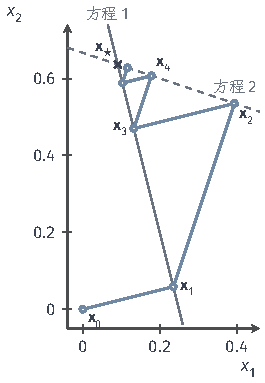
\includegraphics[width=44.81mm]{figures/01-basic-mathematics/03-vectors-matrices-and-multivariate-functions/tikz/c5-kaczmarz-projection-path/figure.pdf}
  \caption{循环Kaczmarz在贯穿例上的交替投影路径。实线为第一个方程$4x_1+x_2=1$的解集，虚线为第二个方程$x_1+3x_2=2$的解集；从$\bm x_0=\bm 0$出发依次垂直投影到两条直线上，折线连接精确计算的前六个迭代点并逐步收拢到交点$\bm x_\star$，图中标出前四个。坐标轴等比例，投影段与对应直线垂直。}
  \label{fig:ls-kaczmarz-projection-path}
\end{figure}

\paragraph{随机选行}
随机版本的投影公式不变，只是选行方式改为按$p_i$独立抽样，收敛结论因此是关于期望的。设方程相容，$\bm x_\star$如定理~\ref{thm:ls-kaczmarz-convergence}，误差$\bm\varepsilon_k$在行空间中。在给定$\bm\varepsilon_k$时对所选行求平均，由式~\eqref{eq:ls-kaczmarz-distance}，
\[
 \begin{aligned}
 \sum_{i=1}^mp_i\frac{(\bm a_i^\top\bm\varepsilon_k)^2}{\lVert\bm a_i\rVert_2^2}
 &=\frac{\lVert\bm A\bm\varepsilon_k\rVert_2^2}{\lVert\bm A\rVert_F^2}\\
 &\geq\frac{\sigma_r^2}{\lVert\bm A\rVert_F^2}\lVert\bm\varepsilon_k\rVert_2^2 ,
 \end{aligned}
\]
其中$\sigma_r$是最小正奇异值，不等号来自定理~\ref{thm:ls-svd-singular-value-norms}对$\ker\bm A$正交补的下界。所以一步之后误差平方的条件平均满足
\[
 \mathbb E\bigl[\lVert\bm\varepsilon_{k+1}\rVert_2^2\bigm|\bm\varepsilon_k\bigr]
 \leq\Bigl(1-\frac{\sigma_r^2}{\lVert\bm A\rVert_F^2}\Bigr)\lVert\bm\varepsilon_k\rVert_2^2 .
\]

选取概率与行的平方范数成正比，正是为了让分母$\lVert\bm a_i\rVert_2^2$被抵消，使这一平均化成$\lVert\bm A\bm\varepsilon_k\rVert_2^2$。

把这一步估计逐步叠加，得到
\begin{equation}
 \mathbb E\lVert\bm\varepsilon_k\rVert_2^2\leq\Bigl(1-\frac{\sigma_r^2}{\lVert\bm A\rVert_F^2}\Bigr)^k\lVert\bm\varepsilon_0\rVert_2^2 ;
 \label{eq:ls-kaczmarz-expected-rate}
\end{equation}
满列秩时这一结论由Strohmer与Vershynin给出\scite{math-strohmer2009randomized}。叠加时需要对此前各次选行的结果取条件期望，所用的随机变量与期望工具可参考\BookChapterRef{chap:random-variables}{卷七第2章“随机变量的分布”}。这里的结论是期望意义下的：单条轨迹上的误差每步不增，但不保证每一步都按这个因子缩小。

\paragraph{不相容情形}
不相容时情况不同。取$\bm A=(1,1)^\top$，$\bm b=(1,3)^\top$，未知量是标量，两行分别要求$x=1$和$x=3$。两行长度都为一，投影化为$x\gets b_i$，循环投影便在$1$与$3$之间往返，而最小二乘解是$\hat x=2$。随机选行时每一步$x$也只取$1$或$3$，所以仅改选行方式不能保证得到最小二乘解。不相容问题交给下一节的算法处理。

图~\ref{fig:solver-inconsistent-row-projections}画出了这个最小的不相容例。每次行投影都使一条方程成立，却始终跨过最小二乘折中点，因而需要校正右端。

\begin{figure}[!htb]
  \centering
  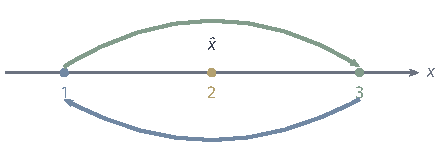
\includegraphics{figures/02-vectors-matrices-and-multivariate-calculus/03-linear-equations-and-optimization/tikz/learning-mechanisms/inconsistent-row-projections.pdf}
  \caption{循环行投影在不相容方程$x=1$、$x=3$之间往返。两条弧形箭头表示依次满足两行后的跳转；黄色点$\hat x=2$是最小二乘解，并非任何一次原始行投影的落点。}
  \label{fig:solver-inconsistent-row-projections}
\end{figure}

\section{扩展Kaczmarz算法}
\label{sec:ls-extended-kaczmarz}

上一节的例子说明，方程不相容时，行投影总在各行的解之间来回，原因是右端含有任何$\bm x$都拟合不了的部分。\term{扩展Kaczmarz算法}（extended Kaczmarz method）先用列投影逐步取出这一部分，再对校正后的相容方程作行投影，从而把Kaczmarz算法推广到一般的最小二乘问题。本节先推导这两种投影及其配合方式，再在上一节的不相容例上逐步执行，最后分析收敛与代价。

\subsection{主要思想}

要解的是最小二乘问题
\[
 \min_{\bm x}\lVert\bm b-\bm A\bm x\rVert_2 ,\qquad \bm A\in\mathbb R^{m\times d},
\]
方程$\bm A\bm x=\bm b$可以不相容，目标是其中范数最小的解$\bm A^\dagger\bm b$。上一节的行投影只适用于相容方程，所以先把问题改写成一个相容方程。

\paragraph{右端的分解}
由正交分解，
\begin{equation}
 \bm b=\bm b_\parallel+\bm b_\perp,\qquad \bm b_\parallel\in\operatorname{range}(\bm A),\quad \bm b_\perp\in\ker(\bm A^\top).
 \label{eq:ls-extended-kaczmarz-rhs-split}
\end{equation}
由第~\ref{sec:ls-ordinary-ls}节，最小二乘解就是相容方程$\bm A\bm x=\bm b_\parallel$的解，其中的最小范数解是$\bm A^\dagger\bm b$；$\bm b_\perp$则是任何$\bm x$都拟合不了的部分。

在不相容例$\bm A=(1,1)^\top$、$\bm b=(1,3)^\top$中，$\operatorname{range}(\bm A)$由$(1,1)^\top$张成。把$\bm b$投影到这条直线上，得
\[
 \bm b_\parallel=\frac{1+3}{2}\begin{bmatrix}1\\1\end{bmatrix}=\begin{bmatrix}2\\2\end{bmatrix}.
\]
剩下的部分是
\[
 \bm b_\perp=\bm b-\bm b_\parallel=\begin{bmatrix}-1\\1\end{bmatrix}.
\]
校正后的方程$\bm A x=\bm b_\parallel$两行都要求$x=2$，正是最小二乘解。

$\bm b_\perp$事先未知，所以引入一个$m$维辅助向量$\bm z$去逼近它，再求解$\bm A\bm x=\bm b-\bm z$。这样就要做两件事：用列的信息把$\bm z$推向$\bm b_\perp$，用行投影求解校正后的方程。

\paragraph{列投影}
$\bm b_\perp$在$\ker(\bm A^\top)$中，即满足$\bm A^\top\bm z=\bm0$：$\bm z$与每一列正交。记第$j$列为$\bm c_j$，这是$d$个齐次方程$\bm c_j^\top\bm z=0$组成的相容方程组，未知量是$\bm z$。把上一节的最短修正用于其中一个方程，就得到一次列投影。

在不相容例中只有一列$\bm c_1=(1,1)^\top$，$\lVert\bm c_1\rVert_2^2=2$。对$\bm z=(z_1,z_2)^\top$，方程的残差为$0-\bm c_1^\top\bm z=-(z_1+z_2)$，最短修正给出
\[
 \bm z-\frac{z_1+z_2}{2}\begin{bmatrix}1\\1\end{bmatrix}
 =\frac12\begin{bmatrix}z_1-z_2\\z_2-z_1\end{bmatrix},
\]
即从每个分量中减去两分量的平均值。从$\bm z=\bm b=(1,3)^\top$出发，一次列投影就得到$(-1,1)^\top=\bm b_\perp$。

一般地，对当前的$\bm z_k$和所选的列$j$，列投影为
\begin{equation}
 \bm z_{k+1}=\bm z_k-\frac{\bm c_j^\top\bm z_k}{\lVert\bm c_j\rVert_2^2}\,\bm c_j .
 \label{eq:ls-extended-kaczmarz-column}
\end{equation}
式中$\bm c_j^\top\bm z_k$衡量$\bm z_k$与第$j$列偏离正交的程度；除以$\lVert\bm c_j\rVert_2^2$换算成沿$\bm c_j$的系数；减去这个倍数之后，$\bm c_j^\top\bm z_{k+1}=0$。它就是对相容方程$\bm A^\top\bm z=\bm0$作一次Kaczmarz投影。

从$\bm z_0=\bm b$出发，每次减去的都是某一列的倍数，属于$\operatorname{range}(\bm A)$。所以$\bm z_k$在$\ker(\bm A^\top)$中的分量始终是$\bm b_\perp$，变化的只是列空间中的部分$\bm z_k-\bm b_\perp$；同时$\bm b-\bm z_k$始终在$\operatorname{range}(\bm A)$中，校正后的方程$\bm A\bm x=\bm b-\bm z_k$始终相容。

\paragraph{校正后的行投影}
若校正量为$\bm z_k$，第$i$条目标方程就是$\bm a_i^\top\bm x=b_i-(\bm z_k)_i$。沿用式~\eqref{eq:ls-kaczmarz-update}的推导，只需把右端$b_i$换成$b_i-(\bm z_k)_i$，得到行投影
\begin{equation}
 \bm x_{k+1}=\bm x_k+\frac{b_i-(\bm z_k)_i-\bm a_i^\top\bm x_k}{\lVert\bm a_i\rVert_2^2}\,\bm a_i .
 \label{eq:ls-extended-kaczmarz-row}
\end{equation}
分子是校正方程第$i$行的行残差，其余与标准Kaczmarz相同。

在不相容例中$\bm a_i=1$，$\lVert\bm a_i\rVert_2^2=1$，行投影化为$x\gets b_i-(\bm z_k)_i$。不作校正（$\bm z=\bm0$）时这就是$x\gets b_i$，在$1$与$3$之间往返；以$\bm z=\bm b_\perp=(-1,1)^\top$校正后，两行分别给出
\[
 1-(-1)=2,\qquad 3-1=2 ,
\]
两行一致，都得到最小二乘解$x=2$。

\paragraph{两种投影的配合}
实际计算中$\bm z_k$只是$\bm b_\perp$的近似，两种投影交替进行。本章采用同步读取轮初状态的版本：每轮的$\bm z_{k+1}$和$\bm x_{k+1}$都由$(\bm z_k,\bm x_k)$计算，行更新不改用刚得到的$\bm z_{k+1}$。先更新$\bm z$、再用新的$\bm z$更新$\bm x$的版本也可以使用，但两种时间顺序产生不同的数值轨迹，实现应与所用的收敛分析一致。行与列的选取沿用上一节的随机规则，这里采用Zouzias与Freris的随机版本\scite{math-zouzias2013randomized}。

于是误差有两个来源。列投影缩小$\bm z_k-\bm b_\perp$；行投影则是在右端仍受这一误差扰动时逼近$\bm A\bm x=\bm b_\parallel$。取$\bm x_0=\bm0$，且每步都沿行方向修正，保证$\bm x_k$始终在行空间中，最终选出最小范数代表。

\subsection{算法实现}

按上一小节的推导，扩展Kaczmarz算法每轮抽取一行和一列，作一次列投影和一次行投影，两者都读取轮初状态；每隔规定的轮数检查两项判据。输入为$\bm A,\bm b$，输出为$\bm x$；超参数为绝对容差$\mathrm{atol}$、相对容差$\mathrm{rtol}$和轮数上限$K$。下面写出变量、初始化与每轮更新。

下面用上一节不相容例的数据逐步演示：
\[
 \bm A=\begin{bmatrix}1\\1\end{bmatrix},\qquad \bm b=\begin{bmatrix}1\\3\end{bmatrix}.
\]
例中取$\mathrm{atol}=0$、$\mathrm{rtol}=0.1$，每轮都作检查。

\paragraph{变量}
\begin{itemize}
 \item $\bm x\in\mathbb R^d$：当前近似解$\bm x_k$。
 \item $\bm z\in\mathbb R^m$：辅助向量$\bm z_k$，逼近不可拟合的部分$\bm b_\perp$；它只是内部状态，不作为输出。
 \item $\lVert\bm a_i\rVert_2^2$与$\lVert\bm c_j\rVert_2^2$：各行、各列的平方范数，预先算好，同时用作抽样权重。
 \item $i_k,j_k$：第$k$轮抽到的行与列。
 \item $\eta_k,\gamma_k$：列投影与行投影的系数，用后即弃。
 \item $k$：轮次，从$0$开始。
\end{itemize}

\paragraph{初始化}
若$\bm A=\bm0$，直接返回最小范数解$\bm x=\bm0$。否则预存各行、各列的平方范数，得到抽样概率
\begin{equation}
 p_i=\frac{\lVert\bm a_i\rVert_2^2}{\lVert\bm A\rVert_F^2},\qquad
 q_j=\frac{\lVert\bm c_j\rVert_2^2}{\lVert\bm A\rVert_F^2};
 \label{eq:ls-extended-kaczmarz-sampling}
\end{equation}
零行和零列的概率为零，不会被抽到，也就不会出现除以零。再把内部状态初始化为
\[
 \bm x_0=\bm0,\qquad \bm z_0=\bm b,\qquad k=0 .
\]
两项判据的阈值按各自的尺度取为
\begin{equation}
 \tau_r=\mathrm{atol}+\mathrm{rtol}\lVert\bm b\rVert_2,\qquad
 \tau_n=\mathrm{atol}+\mathrm{rtol}\lVert\bm A\rVert_F\lVert\bm b\rVert_2 ,
 \label{eq:ls-extended-kaczmarz-thresholds}
\end{equation}
后者的尺度来自$\lVert\bm A^\top\bm z_0\rVert_2=\lVert\bm A^\top\bm b\rVert_2\leq\lVert\bm A\rVert_F\lVert\bm b\rVert_2$。

例中两行的平方范数都为$1$，唯一一列的平方范数为$2$，$\lVert\bm A\rVert_F=\sqrt2$，$\lVert\bm b\rVert_2=\sqrt{10}$，于是
\[
 p_1=p_2=\frac12,\qquad q_1=1 .
\]
两项阈值为
\[
 \tau_r=\frac{\sqrt{10}}{10}\approx0.316,\qquad \tau_n=\frac{\sqrt{20}}{10}\approx0.447 .
\]
初始时$\bm b-\bm z_0-\bm A x_0=\bm0$，但
\[
 \bm A^\top\bm z_0=1+3=4>\tau_n ,
\]
所以进入第一轮。

\paragraph{每轮更新}
在第$k$轮：
\begin{enumerate}
 \item \textbf{抽样。}按概率$p_i$与$q_j$独立抽取行$i_k$和列$j_k$，并记录抽到的行列序列，以便复算同一条轨迹。例中每轮都取$j_k=1$，行$i_k$以各一半的概率取$1$或$2$；下面会看到，两种情况结果相同。

 \item \textbf{列投影。}保存轮初状态$(\bm x_k,\bm z_k)$，按式~\eqref{eq:ls-extended-kaczmarz-column}计算
 \[
  \eta_k=\frac{\bm c_{j_k}^\top\bm z_k}{\lVert\bm c_{j_k}\rVert_2^2},\qquad \bm z_{k+1}=\bm z_k-\eta_k\bm c_{j_k},
 \]
 旧的$\bm z_k$保留给本轮的行投影使用。例中第一轮
 \[
  \eta_0=\frac{1+3}{2}=2 .
 \]
 列投影后的辅助向量为
 \[
  \bm z_1=\begin{bmatrix}1\\3\end{bmatrix}-2\begin{bmatrix}1\\1\end{bmatrix}=\begin{bmatrix}-1\\1\end{bmatrix},
 \]
 已经等于$\bm b_\perp$。

 \item \textbf{行投影。}仍读取旧的$(\bm z_k)_{i_k}$，按式~\eqref{eq:ls-extended-kaczmarz-row}计算
 \[
 \begin{aligned}
  \gamma_k&=\frac{b_{i_k}-(\bm z_k)_{i_k}-\bm a_{i_k}^\top\bm x_k}{\lVert\bm a_{i_k}\rVert_2^2},\\
  \bm x_{k+1}&=\bm x_k+\gamma_k\bm a_{i_k}.
 \end{aligned}
 \]
 例中第一轮用的是$\bm z_0=\bm b$，无论抽到哪一行，分子都是$b_i-b_i-0=0$，所以
 \[
  \gamma_0=0,\qquad x_1=0 ,
 \]
 $x$不动。若行投影改用新的$\bm z_1$，这一步就会提前得到$x=2$；同步版本不这样做。

 \item \textbf{替换状态。}以$(\bm x_{k+1},\bm z_{k+1})$同时替换旧状态，令$k\leftarrow k+1$。

 例中第二轮的列内积为$-1+1=0$，所以
 \[
  \eta_1=0,\qquad \bm z_2=\bm z_1=\begin{bmatrix}-1\\1\end{bmatrix}.
 \]
 行投影读取$\bm z_1$，抽到第一行或第二行时分别得到
 \[
  \gamma_1=1-(-1)-0=2,\qquad \gamma_1=3-1-0=2 .
 \]
 两种情况都得到
 \[
  x_2=2 ,
 \]
 此后不再改变。

 \item \textbf{停止。}在规定的检查轮次，若
 \begin{equation}
  \lVert\bm b-\bm z_k-\bm A\bm x_k\rVert_2\leq\tau_r
  \quad\text{且}\quad
  \lVert\bm A^\top\bm z_k\rVert_2\leq\tau_n ,
  \label{eq:ls-extended-kaczmarz-stopping}
 \end{equation}
 就以“达到容差”结束；若已做满$K$轮，以“次数耗尽”结束；两种情况都取$\bm x=\bm x_k$。

 前一项检查$\bm x_k$对校正方程的拟合，后一项检查辅助向量与列空间的正交性，两项都只是内部停止判据，检查值不作为输出。宣布达到容差之前，再直接计算正规残差$\bm A^\top(\bm b-\bm A\bm x_k)$复核；不要求原残差$\lVert\bm b-\bm A\bm x_k\rVert_2$趋于零。

 例中第一轮后
 \[
  \bm b-\bm z_1-\bm A x_1=\begin{bmatrix}2\\2\end{bmatrix},\qquad \bm A^\top\bm z_1=0 ,
 \]
 后一项已满足，前一项的长度$2\sqrt2\approx2.83$仍大于$\tau_r$，继续。第二轮后
 \[
  \bm b-\bm z_2-\bm A x_2=\bm0,\qquad \bm A^\top\bm z_2=0 ,
 \]
 两项都满足。再复核正规残差，
 \[
  \bm A^\top(\bm b-\bm A x_2)=(1-2)+(3-2)=0 ,
 \]
 以“达到容差”结束。
\end{enumerate}

最终得到
\[
 x_2=2 .
\]
原残差$\bm b-\bm A x_2=(-1,1)^\top$不为零，残差平方和为$2$，正是$\min_x\bigl[(x-1)^2+(x-3)^2\bigr]$的最优值：原方程依然没有精确解，但$x_2=2$已经是最小二乘解。

这个例子也说明两项判据缺一不可：第一轮后$\bm z$已经正确，$x$却还没有移动。

\subsection{算法分析}

\paragraph{极限的含义}
列投影只减去列的倍数，保留$\bm b$的正交残差分量$\bm b_\perp$，同时缩小$\bm z_k-\bm b_\perp$；零初值和沿行方向的修正又使$\bm x_k$始终留在行空间中。当$\bm z_k$趋于$\bm b_\perp$时，行投影求解的就是相容方程$\bm A\bm x=\bm b_\parallel$，而它在行空间中的唯一解是$\bm A^\dagger\bm b$，所以这一构造指向最小范数最小二乘解。

\paragraph{列校正的收敛}
列投影是对相容方程$\bm A^\top\bm z=\bm 0$作Kaczmarz投影，初值为$\bm b$。由定理~\ref{thm:ls-kaczmarz-convergence}（对$\bm A^\top$应用），按固定循环顺序选列时，$\bm z_k$收敛到$\bm b$在$\ker(\bm A^\top)$上的正交投影，即$\bm b_\perp$，每轮按小于一的因子几何收缩。随机选列时，上一节的一步平均估计同样适用于$\bm z_k-\bm b_\perp$，它属于$\operatorname{range}(\bm A)$，平均缩小因子为$1-\sigma_r^2/\lVert\bm A\rVert_F^2$。

\paragraph{行迭代的误差递推}
令$\bm x_\star=\bm A^\dagger\bm b$，它满足$\bm A\bm x_\star=\bm b_\parallel=\bm b-\bm b_\perp$，故$b_i=\bm a_i^\top\bm x_\star+(\bm b_\perp)_i$。代入行投影，误差$\bm\varepsilon_k=\bm x_k-\bm x_\star$满足
\begin{equation}
 \bm\varepsilon_{k+1}=\bm P_{i_k}\bm\varepsilon_k+\frac{(\bm b_\perp-\bm z_k)_{i_k}}{\lVert\bm a_{i_k}\rVert_2^2}\,\bm a_{i_k}.
 \label{eq:ls-extended-kaczmarz-error-recursion}
\end{equation}
第一项是标准Kaczmarz的误差映射，第二项是校正误差带来的扰动，长度不超过$\lVert\bm z_k-\bm b_\perp\rVert_2/\lVert\bm a_{i_k}\rVert_2$。$\bm\varepsilon_k$始终在行空间中。

在循环版本中，把一轮行扫掠合起来，有
\begin{equation}
 \lVert\bm\varepsilon_{\text{轮末}}\rVert_2\leq q\lVert\bm\varepsilon_{\text{轮初}}\rVert_2+\varphi ,
 \label{eq:ls-extended-kaczmarz-sweep-bound}
\end{equation}
其中$q<1$是定理~\ref{thm:ls-kaczmarz-convergence}中的因子，$\varphi$是本轮各步扰动长度之和，随$\bm z_k\to\bm b_\perp$趋于零。由这一递推，轮末误差有界；记其上极限为$L$，则$L\leq qL$，故$L=0$，即$\bm x_k\to\bm A^\dagger\bm b$。

随机版本在规定的独立抽样下，期望平方误差以由$1-\sigma_r^2/\lVert\bm A\rVert_F^2$决定的几何速率趋于零\scite{math-zouzias2013randomized}，证明同样要用条件期望。这里不宣称每条轨迹的原残差逐步下降，算法实现的例子中第一轮$x$就完全没有移动。

\paragraph{代价}
每轮访问一行、一列，并保存长度为$m$的$\bm z_k$，代价按访问的非零元个数计算；停止检查需要计算$\bm A\bm x_k$与$\bm A^\top\bm z_k$，各相当于一次完整的矩阵乘向量，所以只按规定间隔进行。数值敏感性仍受原问题小奇异值的影响：两种收缩因子都由$\sigma_r^2/\lVert\bm A\rVert_F^2$决定，它很小时收敛很慢。

\section{本章小结}
\label{sec:row-projection-summary}

本章回答了只能逐行或逐列访问数据时怎样求解线性方程。Kaczmarz算法每次只满足一个方程：由最短修正原理，更新沿所选行的法向进行，系数由行残差除以行的平方范数确定，新点是当前点到该超平面的正交投影。方程相容时，每一步到每个精确解的距离都不增；循环版本每轮按小于一的因子收缩，收敛到$\bm A^\dagger\bm b$加上初值的零空间分量，零初值时就是最小范数解。随机版本按行的平方范数抽样，期望平方误差以$1-\sigma_r^2/\lVert\bm A\rVert_F^2$为因子几何减小。

使用时要注意几个条件。行之间越接近平行，收敛越慢；零行对应非零右端说明方程不相容，必须单独处理；某一行的残差为零不说明求解完成。方程不相容时，标准Kaczmarz在各行的解之间往返，无论循环还是随机选行，都不会停在最小二乘解上。

扩展Kaczmarz算法把右端分成可拟合与不可拟合两部分：列投影从$\bm z_0=\bm b$出发逼近不可拟合的$\bm b_\perp$，行投影求解校正后的相容方程$\bm A\bm x=\bm b-\bm z$。本章采用同步版本，两种投影都读取轮初状态；零初值保证极限是最小范数最小二乘解。

检验时，标准算法看全部方程的原残差；扩展算法看$\lVert\bm A^\top\bm z\rVert_2$与校正方程的残差，并复核正规残差，原残差最终非零是正常的。两种算法的最小范数性质都依赖零初值和行空间保持，不由残差判据保证。它们每步只读一行或一列，代价低，但收敛速度受$\sigma_r^2/\lVert\bm A\rVert_F^2$限制；误差解释与方法比较在第~\ref{chap:solution-error-regularization}章进行。
